\documentclass{standalone}
\usepackage{tikz}
\usetikzlibrary{patterns, positioning}


\begin{document}
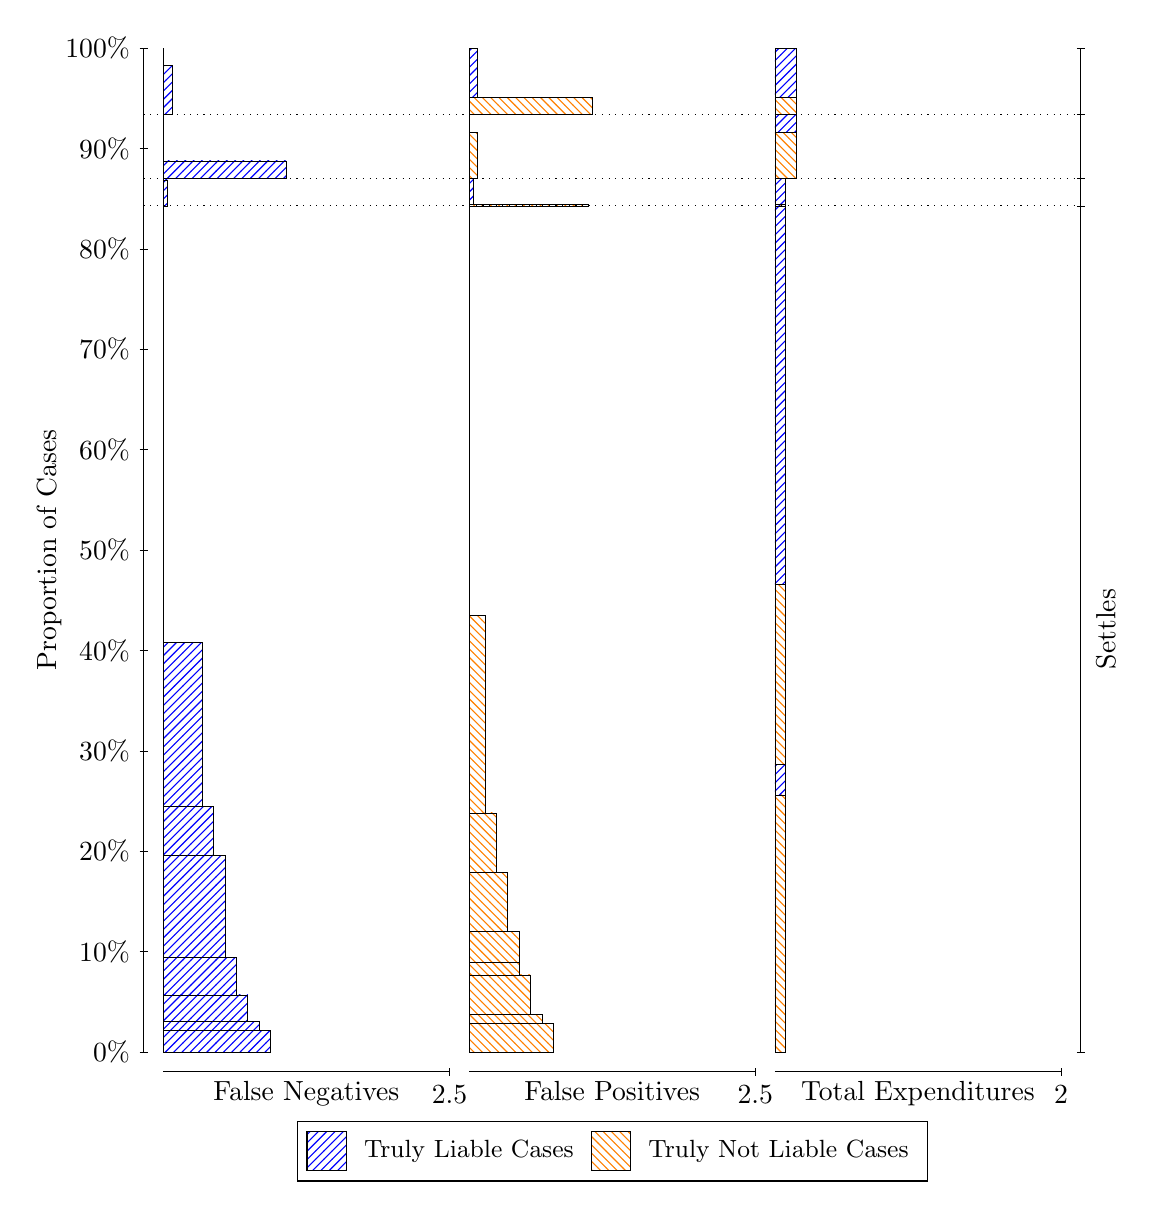
\begin{tikzpicture}
\draw[black, very thin] (1.5,1.75) -- (1.5,14.5);
\node[rotate=90, text=black, anchor=center] at (0.3, 8.125) {Proportion of Cases};
\draw[black, very thin] (1.45,1.75) -- (1.55,1.75);
\node[text=black, anchor=east] at (1.45, 1.75) {0\%};
\draw[black, very thin] (1.45,3.025) -- (1.55,3.025);
\node[text=black, anchor=east] at (1.45, 3.025) {10\%};
\draw[black, very thin] (1.45,4.3) -- (1.55,4.3);
\node[text=black, anchor=east] at (1.45, 4.3) {20\%};
\draw[black, very thin] (1.45,5.575) -- (1.55,5.575);
\node[text=black, anchor=east] at (1.45, 5.575) {30\%};
\draw[black, very thin] (1.45,6.85) -- (1.55,6.85);
\node[text=black, anchor=east] at (1.45, 6.85) {40\%};
\draw[black, very thin] (1.45,8.125) -- (1.55,8.125);
\node[text=black, anchor=east] at (1.45, 8.125) {50\%};
\draw[black, very thin] (1.45,9.4) -- (1.55,9.4);
\node[text=black, anchor=east] at (1.45, 9.4) {60\%};
\draw[black, very thin] (1.45,10.675) -- (1.55,10.675);
\node[text=black, anchor=east] at (1.45, 10.675) {70\%};
\draw[black, very thin] (1.45,11.95) -- (1.55,11.95);
\node[text=black, anchor=east] at (1.45, 11.95) {80\%};
\draw[black, very thin] (1.45,13.225) -- (1.55,13.225);
\node[text=black, anchor=east] at (1.45, 13.225) {90\%};
\draw[black, very thin] (1.45,14.5) -- (1.55,14.5);
\node[text=black, anchor=east] at (1.45, 14.5) {100\%};

\draw[black, very thin] (13.4,1.75) -- (13.4,14.5);
\draw[black, very thin] (13.35,1.75) -- (13.45,1.75);
\node[anchor=west] at (13.35, 1.75) {};
\draw[black, very thin] (13.35,12.495) -- (13.45,12.495);
\node[anchor=west] at (13.35, 12.495) {};
\draw[black, very thin] (13.35,12.847) -- (13.45,12.847);
\node[anchor=west] at (13.35, 12.847) {};
\draw[black, very thin] (13.35,13.653) -- (13.45,13.653);
\node[anchor=west] at (13.35, 13.653) {};
\draw[black, very thin] (13.35,14.5) -- (13.45,14.5);
\node[anchor=west] at (13.35, 14.5) {};

\draw[black, very thin, pattern color=blue, pattern=north east lines] (1.75,1.75) rectangle (3.1125,2.0193);
\draw[black, very thin, pattern color=blue, pattern=north east lines] (1.75,2.0193) rectangle (2.9672,2.1388);
\draw[black, very thin, pattern color=blue, pattern=north east lines] (1.75,2.1388) rectangle (2.8218,2.4751);
\draw[black, very thin, pattern color=blue, pattern=north east lines] (1.75,2.4751) rectangle (2.6765,2.949);
\draw[black, very thin, pattern color=blue, pattern=north east lines] (1.75,2.949) rectangle (2.5312,4.2477);
\draw[black, very thin, pattern color=blue, pattern=north east lines] (1.75,4.2477) rectangle (2.3858,4.868);
\draw[black, very thin, pattern color=blue, pattern=north east lines] (1.75,4.868) rectangle (2.2405,6.9496);
\draw[black, very thin, pattern color=orange, pattern=north west lines] (1.75,6.9496) rectangle (1.75,12.495);
\draw[black, very thin, pattern color=blue, pattern=north east lines] (1.75,12.495) rectangle (1.8045,12.824);
\draw[black, very thin, pattern color=orange, pattern=north west lines] (1.75,12.824) rectangle (1.75,12.847);
\draw[black, very thin, pattern color=blue, pattern=north east lines] (1.75,12.847) rectangle (3.3123,13.068);
\draw[black, very thin, pattern color=orange, pattern=north west lines] (1.75,13.068) rectangle (1.75,13.653);
\draw[black, very thin, pattern color=blue, pattern=north east lines] (1.75,13.653) rectangle (1.859,14.278);
\draw[black, very thin, pattern color=orange, pattern=north west lines] (1.75,14.278) rectangle (1.75,14.5);
\draw[black, very thin, pattern color=orange, pattern=north west lines] (5.6333,1.75) rectangle (6.7052,2.1104);
\draw[black, very thin, pattern color=orange, pattern=north west lines] (5.6333,2.1104) rectangle (6.5598,2.231);
\draw[black, very thin, pattern color=orange, pattern=north west lines] (5.6333,2.231) rectangle (6.4145,2.7296);
\draw[black, very thin, pattern color=orange, pattern=north west lines] (5.6333,2.7296) rectangle (6.2692,2.8858);
\draw[black, very thin, pattern color=orange, pattern=north west lines] (5.6333,2.8858) rectangle (6.2692,3.2795);
\draw[black, very thin, pattern color=orange, pattern=north west lines] (5.6333,3.2795) rectangle (6.1238,4.0315);
\draw[black, very thin, pattern color=orange, pattern=north west lines] (5.6333,4.0315) rectangle (5.9785,4.7862);
\draw[black, very thin, pattern color=orange, pattern=north west lines] (5.6333,4.7862) rectangle (5.8332,7.2953);
\draw[black, very thin, pattern color=blue, pattern=north east lines] (5.6333,7.2953) rectangle (5.6333,12.495);
\draw[black, very thin, pattern color=orange, pattern=north west lines] (5.6333,12.495) rectangle (7.1412,12.517);
\draw[black, very thin, pattern color=blue, pattern=north east lines] (5.6333,12.517) rectangle (5.6878,12.847);
\draw[black, very thin, pattern color=orange, pattern=north west lines] (5.6333,12.847) rectangle (5.7423,13.432);
\draw[black, very thin, pattern color=blue, pattern=north east lines] (5.6333,13.432) rectangle (5.6333,13.653);
\draw[black, very thin, pattern color=orange, pattern=north west lines] (5.6333,13.653) rectangle (7.1957,13.876);
\draw[black, very thin, pattern color=blue, pattern=north east lines] (5.6333,13.876) rectangle (5.7423,14.5);
\draw[black, very thin, pattern color=orange, pattern=north west lines] (9.5167,1.75) rectangle (9.6529,5.0138);
\draw[black, very thin, pattern color=blue, pattern=north east lines] (9.5167,5.0138) rectangle (9.6529,5.4026);
\draw[black, very thin, pattern color=orange, pattern=north west lines] (9.5167,5.4026) rectangle (9.6529,7.6841);
\draw[black, very thin, pattern color=blue, pattern=north east lines] (9.5167,7.6841) rectangle (9.6529,12.495);
\draw[black, very thin, pattern color=orange, pattern=north west lines] (9.5167,12.495) rectangle (9.6529,12.517);
\draw[black, very thin, pattern color=blue, pattern=north east lines] (9.5167,12.517) rectangle (9.6529,12.847);
\draw[black, very thin, pattern color=orange, pattern=north west lines] (9.5167,12.847) rectangle (9.7892,13.432);
\draw[black, very thin, pattern color=blue, pattern=north east lines] (9.5167,13.432) rectangle (9.7892,13.653);
\draw[black, very thin, pattern color=orange, pattern=north west lines] (9.5167,13.653) rectangle (9.7892,13.876);
\draw[black, very thin, pattern color=blue, pattern=north east lines] (9.5167,13.876) rectangle (9.7892,14.5);
\draw[black, dotted] (1.5,12.495) -- (13.4,12.495);
\draw[black, dotted] (1.5,12.847) -- (13.4,12.847);
\draw[black, dotted] (1.5,13.653) -- (13.4,13.653);
\draw[black, very thin] (1.75,1.5) -- (5.3833,1.5);
\node[text=black, anchor=north] at (3.5667, 1.5) {False Negatives};
\draw[black, very thin] (5.3833,1.45) -- (5.3833,1.55);
\node[text=black, anchor=north] at (5.3833, 1.45) {2.5};

\draw[black, very thin] (5.6333,1.5) -- (9.2667,1.5);
\node[text=black, anchor=north] at (7.45, 1.5) {False Positives};
\draw[black, very thin] (9.2667,1.45) -- (9.2667,1.55);
\node[text=black, anchor=north] at (9.2667, 1.45) {2.5};

\draw[black, very thin] (9.5167,1.5) -- (13.15,1.5);
\node[text=black, anchor=north] at (11.333, 1.5) {Total Expenditures};
\draw[black, very thin] (13.15,1.45) -- (13.15,1.55);
\node[text=black, anchor=north] at (13.15, 1.45) {2};

\node[text=black, centered, rotate=90] at (13.72, 7.1225) {Settles};




\draw (7.449999999999999,1.5) node[draw=none] (baseCoordinate) {};
\begin{scope}[align=center]
        \matrix[scale=0.5, draw=black, below=0.5cm of baseCoordinate, nodes={draw}, column sep=0.1cm]{
            \node[rectangle, draw, minimum width=0.5cm, minimum height=0.5cm, pattern color=blue, pattern=north east lines] {}; &
            \node[draw=none, font=\small, text=black] (B) {Truly Liable Cases}; &
            \node[rectangle, draw, minimum width=0.5cm, minimum height=0.5cm, pattern color=orange, pattern=north west lines] {}; &
            \node[draw=none, font=\small, text=black] (B) {Truly Not Liable Cases}; \\
            };
\end{scope}

\end{tikzpicture}
\end{document}